\section{Least squares as orthogonal projection}
\label{sec:projection}

We observe $n$ pairs $(x_i, y_i)$ and assume $X \in \mathbb{R}^{n \times k}$
has \textbf{full column rank}. The model is
\begin{equation}
    y = X\beta + \varepsilon, \qquad \mathbb{E}[\varepsilon \mid X] = 0 .
    \label{eq:model}
\end{equation}

\begin{theorem}[Orthogonal projection]\label{thm:projection}
Let $S \subseteq \mathbb{R}^n$ be a subspace. There is a unique $\hat y \in S$
minimising $\|y - s\|$ over $s \in S$, and $y - \hat y \perp S$.
\end{theorem}

\begin{proof}
For any $s \in S$, Pythagoras gives
\begin{align}
    \|y - s\|^2 &= \|y - \hat y\|^2 + \|\hat y - s\|^2 \label{eq:pythagoras} \\
                &\ge \|y - \hat y\|^2 .
\end{align}
\end{proof}

\begin{corollary}[Normal equations]\label{cor:normal}
Under \eqref{eq:model}, Theorem \ref{thm:projection} with
$S = \operatorname{col}(X)$ gives
\begin{equation}
    \hat\beta = (X^\top X)^{-1} X^\top y .
    \label{eq:normal}
\end{equation}
\end{corollary}

Three things follow from \eqref{eq:normal}:
\begin{itemize}
    \item the residuals $e = y - X\hat\beta$ are orthogonal to every regressor;
    \item $\hat y = Py$ with $P = X(X^\top X)^{-1} X^\top$ idempotent;
    \item with an intercept, the residuals sum to zero.
\end{itemize}

\begin{figure}[ht]
    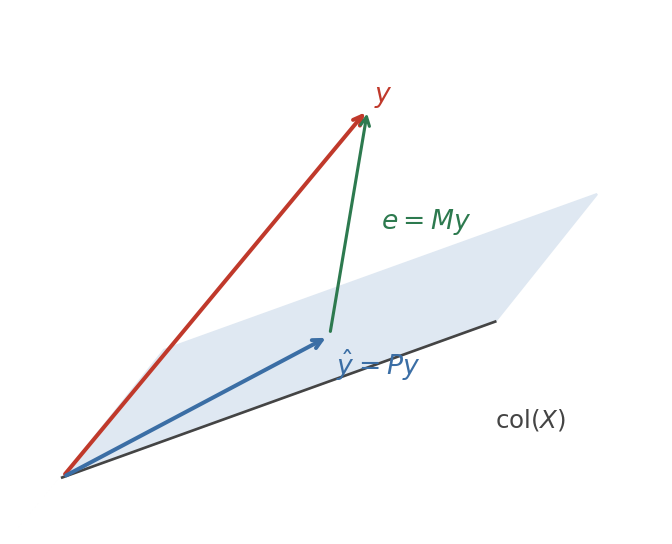
\includegraphics[width=0.5\textwidth]{figures/projection.png}
    \caption{The fit is the projection of $y$ onto the column space of $X$.}
    \label{fig:projection}
\end{figure}

